% !TEX root = widefieldscan.tex
\svnidlong
{$HeadURL$}
{$LastChangedDate$}
{$LastChangedRevision$}
{$LastChangedBy$}
%
\section{Materials and Methods}
\label{sec:materials and methods}
\subsection{Sample Preparation}
Rat lung samples, prepared according to
\ifhtml
	\citet{Tschanz2002} and \citet{Luyet2002}
\else
	\citeasnoun{Tschanz2002} and \citeasnoun{Luyet2002}
\fi
were used as test objects. Briefly, lungs of Sprague-Dawley rats were filled with \SI{2.5}{\percent} glutaraldehyde (\cf{CH2(CH2CHO)2}) in \SI{0.03}{\Molar} potassium-phosphate buffer (pH 7.4) by instillation via tracheotomy at a constant pressure of \SI{20}{\centi\meter} water column. In order to prevent recoiling of the lung, this pressure was maintained during glutaraldehyde-fixation for a minimum of two hours. Subsequently, the lungs were dissected free and immersed in toto in the same fixative at a temperature of \SI{4}{\celsius} for at least \SI{24}{\hour}.

The samples were postfixed with \SI{1}{\percent} osmium tetroxide (\cf{OsO4}) and stained with \SI{4}{\percent} uranyl nitrate (\cf{UO2(NO3)2}) to increase the x-ray absorption contrast, dehydrated in a graded series of ethanol and embedded in paraffin using Histoclear (Merck KGaA, Darmstadt, Germany) as an intermedium. The lung samples were mounted onto standard scanning electron microscopy sample holders (PLANO GmbH, Wetzlar, Germany) using paraffin~\cite{Tsuda2008}.

The handling of animals before and during the experiments, as well as the experiments themselves, were approved and supervised by the Swiss Agency for the Environment, Forests and Landscape and the Veterinary Service of the Canton of Bern, Switzerland.

\subsection{Synchrotron radiation tomographic microscopy}
The experiments were performed on the TOMCAT beamline at the Swiss Light Source, Paul Scherrer Institut, Villigen, Switzerland. The samples were scanned at \SI{12.6}{\kilo\electronvolt}. After penetration through the sample, the x-rays were converted into visible light by a YAG:Ce scintillator (\SI{18}{\micro\meter} thickness, Crismatec Saint-Gobain, Nemours, France). The projections were magnified by diffraction limited microscope optics (10$\times$ magnification) and digitized by a high-resolution 2048$\times$2048 pixel CCD camera (pco.2000, PCO AG, Kelheim, Germany) with 14 bit dynamic range. The detector was operated in 2$\times$2 binning mode, as a result, the pixel size was \SI{1.48}{\micro\meter} and the exposure time was \SI{175}{\milli\second}.

Projections $I_{Pr}$, were recorded at equiangular positions between \SI{0}{\degree} and \SI{180}{\degree}. The exact number of angular projections depended on the selected scan protocol, as described in section~\ref{subsec:increasing the field of view}. Additionally, for each protocol a set of dark ($I_{D}$) and flat images ($I_{F}$) were recorded for noise and baseline correction, respectively. Further details can be found in 
\ifhtml
	\citet{Hintermueller2010}
\else
	\citeasnoun{Hintermueller2010}
\fi%
.

\subsection{Increasing the field of view}\label{subsec:increasing the field of view}
For parallel beam geometry, tomographic images are obtained at equidistant angles over a sample rotation of \SI{180}{\degree} as shown in Figure~\ref{fig:scanning-possibilities}(a). After reconstruction, the width of the image corresponds to the field of view of the camera.

Samples twice as large as the field of view can be imaged using scanning protocols based on a \SI{360}{\degree} off center sample rotation as shown in Figure~\ref{fig:scanning-possibilities}(b). Images recorded between \SI{180}{\degree} and \SI{360}{\degree} have to be flipped after acquisition: the projections obtained at angular position $\theta$ and $\theta$+\SI{180}{\degree} ($I_{Pr_{\theta}}$ and $I_{Pr_{\theta+\SI{180}{\degree}}}$) have to be stitched to one projection. The resulting images cover twice the field of view of the camera.

\begin{figure}
	\centering
	\caption{Covering the field of view of differently sized samples with one \SI{180}{\degree} scan (a), one \SI{360}{\degree} scan (b) or---in the case of the so called wide field scanning---with multiple subscans (three subscans, c). The filled segments mark the region of the sample that is covered while scanning the respective positions (Position 1: magenta/checkerboard, Position 2: yellow, Position 3: cyan/striped).}%
	\ifiucr		
		%\documentclass{article}
%\usepackage[demo]{graphicx}
%\usepackage{subfig}
%\usepackage{tikz}
%\usepackage{multirow}
%\usepackage{siunitx}
%\begin{document}
%\begin{figure}
%%%%%%%%%%%%%%%%%%%%%%%%%%%%%
%\begin{tabular}{cc}
%Fig A & \multirow{3}{*}{Fig D}\\
%Fig B & \\
%Fig C & \\
%\end{tabular}
\noindent\makebox[\textwidth]{%
\begin{tabular}{cc}
%%%%% LEFT TOP %%%%%
	\subfloat[\SI{180}{\degree-scan}]{
		%%%%%
		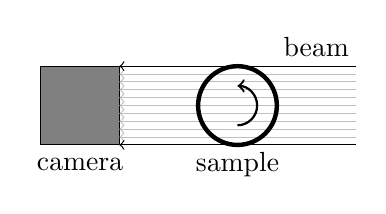
\begin{tikzpicture}
			%drawing grid
			%\draw[color=gray] (0,0) grid (8,1);
			\def\start{0}
			\def\length{1}
			%camera
			\draw [fill=gray] (\start,\start) rectangle (\length,\length);
			\node at (.5*\length,-.25) {camera};
			% beam
			\foreach \x in {0,.1,...,1.1}
				\draw[gray!50,<-] (\length,\x) -- (4*\length,\x);
			\foreach \x in {0,\length}
				\draw[<-] (\length,\x) -- (4*\length,\x);
			\node at (3.5*\length,\length+.25) {beam};
			%sample
			\draw[ultra thick] (2.5*\length,0.5*\length) circle (.5*\length);
			\draw[thick,->] (2.5*\length,0.25*\length) arc (-90:90:.25*\length);
			\node at (2.5*\length,-.25) {sample};
		\end{tikzpicture}
		%%%%%
		\label{subfig:180degreescan}
	}%
& %%%%% RIGHT TOP %%%%%
	\multirow{3}{*}{%
	\subfloat[Stacked scanning for long and thin samples]{
		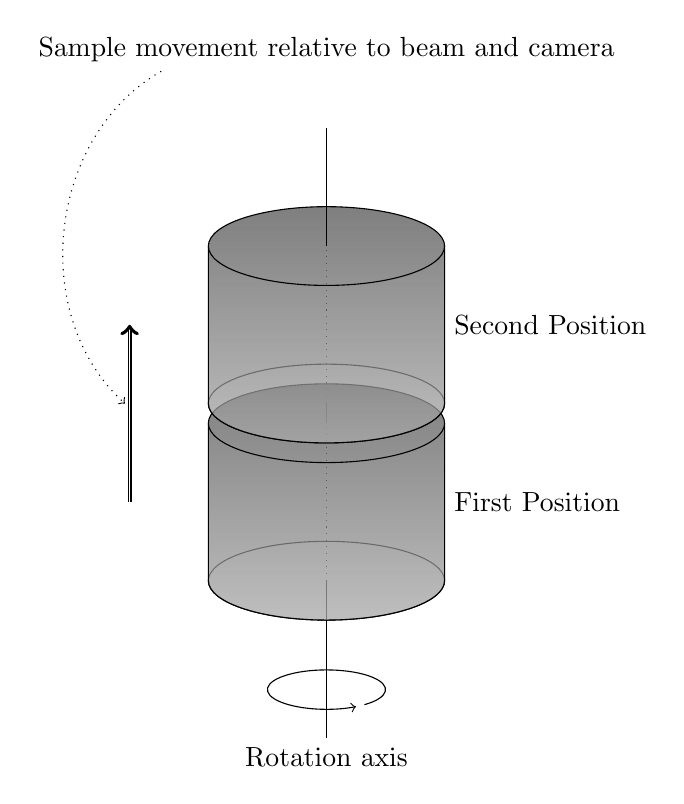
\begin{tikzpicture}%[ultra thick,scale=1]%,show background grid]
			%draw axes
				%\draw[ultra thick] (-10,0) -- (10,0);
				%\draw[ultra thick] (0,-10) -- (0,10);
				%\draw[ultra thick] (0,0) circle (.125);
			% rotation axis
				\draw[->] (0,-2) ++ (-50:.75) arc (-50:300:.75 and .25);
				\draw (0,-3) node [below] {Rotation axis} -- ++(0,2);
				\draw[dotted] (0,-1) -- ++(0,2);
				\draw (0,1) -- ++(0,0.25);
				\draw[dotted] (0,1.25) -- ++(0,2);
			% position 1
				\draw (0,-1) circle (1.5 and .5);
				\fill[shade,semitransparent] (-1.5,-1) arc (-180:0:1.5 and .5) -- ++(0,2) arc (0:180:1.5 and .5) -- cycle;
				\draw (-1.5,-1) arc (-180:0:1.5 and .5) -- ++(0,2) arc (0:180:1.5 and .5) -- cycle;		
				\draw (-1.5,1) arc (-180:0:1.5 and .5);
				\draw (1.5,0) node [right] {First Position};
			% position 2
				\draw (0,1.25) circle (1.5 and .5);
				\fill[shade,semitransparent] (-1.5,1.25) arc (-180:0:1.5 and .5) -- ++(0,2) arc (0:180:1.5 and .5) -- cycle;
				\draw (-1.5,1.25) arc (-180:0:1.5 and .5) -- ++(0,2) arc (0:180:1.5 and .5) -- cycle;		
				\draw (-1.5,3.25) arc (-180:0:1.5 and .5);
				\draw (1.5,2.25) node [right] {Second Position};
			% rotation axis on top
				\draw (0,3.25) -- ++(0,1.5);									
			% sample movement
				\draw[double,->] (-2.5,0) -- (-2.5,2.25) ;% node [text width=10cm,midway,left] {Sample movement relative to beam and camera};	
				% sample movement
				\node (movefrom) at (0,5.75) {Sample movement relative to beam and camera};
				\node (moveto) at (-2.5,1.125) {};
				\draw [->,dotted] (movefrom) to [bend right=54] (moveto);
		\end{tikzpicture}
		\label{subfig:stackedscan}
	}%
	}
\\
%%%%% LEFT MIDDLE %%%%%	
	\subfloat[\SI{360}{\degree-scan}]{
		%%%%%
		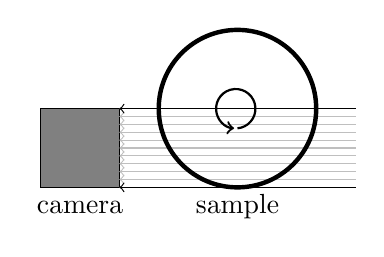
\begin{tikzpicture}
			%drawing grid
			%\draw[color=gray] (0,0) grid (8,1);
			\def\start{0}
			\def\length{1}
			%camera
			\draw [fill=gray] (\start,\start) rectangle (\length,\length);
			\node at (.5*\length,-.25) {camera};
			% beam
			\foreach \x in {0,.1,...,1.1}
				\draw[gray!50,<-] (\length,\x) -- (4*\length,\x);
			\foreach \x in {0,\length}
				\draw[<-] (\length,\x) -- (4*\length,\x);
		%	\node at (3.5*\length,\length+.25) {beam};
			%sample
			\draw[ultra thick] (2.5*\length,\length) circle (\length);
			\draw[thick,->] (2.5*\length,\length-0.25*\length) arc (-85:265:0.25*\length);
			\node at (2.5*\length,-.25) {sample};
		\end{tikzpicture}
		%%%%%
		\label{subfig:360degreescan}
	}%
& %%%%% RIGHT MIDDLE %%%%%
\\
%%%%% LEFT BOTTOMT %%%%%
	\subfloat[wide field scan]{
		%%%%%
		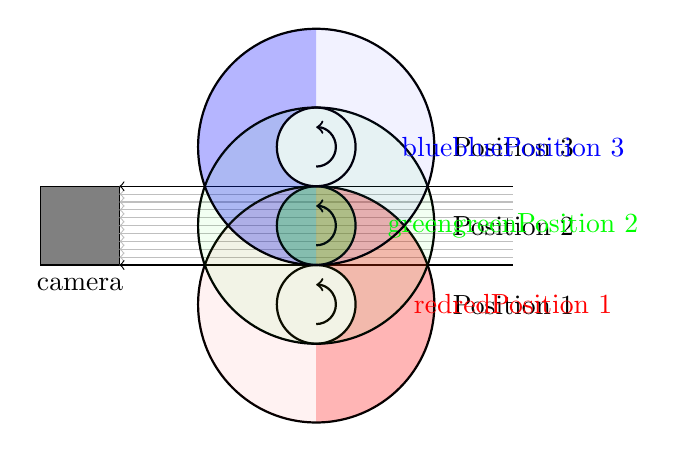
\begin{tikzpicture}
			\def\length{1}
			\def\beamlength{6}
			%grid
		%	\draw[color=gray] (0,-3) grid (7,3);
			%camera
			\draw [fill=gray] (0,0) rectangle (\length,\length);
			\node at (.5*\length,-.25) {camera};
			% beam
			\foreach \x in {0,.1,...,1.1}
				\draw[gray!50,<-] (\length,\x) -- (\beamlength,\x);
			\foreach \x in {0,\length}
				\draw[<-] (\length,\x) -- (\beamlength,\x);
		%	\node at (3.5*\length,\length+.25) {beam};
		%%%%%	%colored samples
		%%%%%	\foreach \y/\color/\position in {-.5/red/1,.5/green/2,1.5/blue/3}
		%%%%%		{
		%%%%%			\draw[thick,color=\color] (0.5*\beamlength+0.5*\length,\y) circle (1.5*\length) circle (.5*\length);
		%%%%%			\draw[thick,->,color=\color] (0.5*\beamlength+0.5*\length,\y-.25*\length) arc (-90:90:0.25*\length);
		%%%%%			\node[color=\color] at (\beamlength,\y) {Position \position};
		%%%%%		}
			% filled samples
			\fill [color=red,nearly transparent]   (3.5,1) arc (90:-90:1.5*\length) -- ++(0,1) arc (-90:90:.5*\length);
			\fill [color=blue,nearly transparent]  (3.5,3) arc (90:270:1.5*\length) -- ++(0,1) arc (270:90:.5*\length);
			\fill [color=green,nearly transparent] (0.5*\beamlength+0.5*\length,.5) circle (0.5*\length);	
			\foreach \y/\position/\color in {-.5/1/red,.5/2/green,1.5/3/blue}
				{
					\draw[thick] (0.5*\beamlength+0.5*\length,\y) circle (1.5*\length) circle (.5*\length);
					\draw[thick,->] (0.5*\beamlength+0.5*\length,\y-.25*\length) arc (-90:90:0.25*\length);
					\fill [color=\color,ultra nearly transparent] (0.5*\beamlength+0.5*\length,\y) circle (1.5*\length);
					\node at (\beamlength+.005,\y-.005) {Position \position};
					\node [color=\color] at (\beamlength,\y) {Position \position};
				}
		\end{tikzpicture}
		%%%%%
		\label{subfig:widefieldscan}
	}%
& %%%%% RIGHT BOTTOM %%%%%
\\
\end{tabular}
} %makebox
%%%%%%%%%%%%%%%%%%%%%%%%%%%%%	
%\caption{Caption of subfigures \subref{subfig:180degreescan}, \subref{subfig:360degreescan}, \subref{subfig:widefieldscan} and \subref{subfig:stackedscan}}
%\end{figure}
%\end{document}%
	\else
	\fi
	\label{fig:scanning-possibilities}%
\end{figure}

For tomographic scans covering a size wider than two fields of view, three or more \SI{180}{\degree}-scans taken at slightly overlapping positions are combined, as shown Figure~\ref{fig:scanning-possibilities}(c). The projections of each subscan overlap slightly to facilitate the stitching of multiple projections into a single one. The cutline, \ie the position where the merging takes place, is automatically determined according to a mean squared difference method~\cite{Hintermueller2010}.

A straightforward acquisition scheme would record an equal amount of projections for each of the individual subscans. As a consequence of fulfilling the sampling theorem in the lateral parts of the sample we would thus oversample the central parts of the sample. 

Since the total acquisition time per sample linearly scales with the total amount of recorded projections such an acquisition scheme obviously increases the total amount of beamtime for one sample without relevantly increasing the quality of the reconstructed tomographic data. Thus, such an oversampling is generally avoided.

Our goal was to find a good compromise between scanning time and image quality. We thus devised an acquisition scheme for covering a wide field of view based on the assumption that a sufficient resolution and contrast can be achieved in the tomographic dataset, if the sampling theorem is individually fulfilled for each of the subscans. This results in a set of $i$ subscans with $P_{i}$ projections each. A simple example with $P_{2}=4$ and $P_{1}=P_{3}=8$ is shown in Figure~\ref{fig:projections}(a). Since each subscan $i$ has a different number of projections $P_{i}$, the stitching algorithm has to interpolate missing projections from adjacent projections (represented by the dotted lines in Figure~\ref{fig:projections}(b)) to generate a complete set of merged projections for reconstruction.

As a by-product, such an optimization of the individual number of projections $P_{i}$ for each subscan $i$ decreases the total acquisition time for one sample and thus the imparted radiation dose.

\begin{figure}
	\centering
	\caption{Wide field scan setup with three \SI{180}{\degree} scans; one central (yellow, central) and two lateral scans (magenta and cyan or top and bottom, respectively). In this drawing, four projections for the central and eight projections for each of the lateral scans have been chosen. The colors of the three positions correspond to the colors shown in Figure~\ref{fig:scanning-possibilities}(c). Panel a): scanned projections, panel b): scanned projections and additional interpolated projections (dotted) required to merge all projections.}
	\ifiucr
		%\documentclass{article}
%\usepackage[demo]{graphicx}
%\usepackage{subfig}
%\usepackage{tikz}
%\usepackage{multirow}
%\usepackage{siunitx}
%\begin{document}
%\begin{figure}
%\centering
%%%%%%%%%%%%%%%%%%%%%%%%%%%%%
\def\radius{1}%
\def\gap{0.05}%
\begin{tikzpicture}[ultra thick,scale=.618]%
	\foreach \ang in {0,45,...,359}%
		{%
		\draw [color=green] (\ang:0) -- (\ang:\radius);%
		}%
	\foreach \ang in {0,22.5,...,179}%
		{%
		\draw [color=red] (\ang:\radius+\gap) -- (\ang:3*\radius+\gap);%
		}%
	\foreach \ang in {180,202.5,...,359}%
		{%
		\draw [color=blue] (\ang:\radius+\gap) -- (\ang:3*\radius+\gap);%
		}%
	\node [anchor=south west] at (-3.05,-3.05) {(a)};
\end{tikzpicture}
%%%%%%%%%%%%%%%%%%%%%%%%%%%%%	
%\caption{Projection Setup}
%\end{figure}
%\end{document}%
		\input{tikz-images/ProjectionSetupInterpolate}
	\else
	\fi
	\label{fig:projections}
\end{figure}	

We defined a gold standard protocol and several additional scanning protocols in order to compare different acquisition schemes. The gold standard protocol covers the desired field of view while fulfilling the sampling theorem (which states that for a detector width of $D$ pixels, we need to acquire a number of projections $P=D\frac{\pi}{2}$~\cite{Kak2002}) in all its regions, as shown in Figure~\ref{fig:SubScan-Setup}(a). In this case we need to achieve a field of view of 3072 pixels. The dark gray circle is the field of view that could be covered using a detector with a diameter of 3072 pixels.

Using a detector with a size of 1024 pixels, this desired field of view could be covered with nine independent local tomography scans. Such an approach would require nine independent reconstructions and stitching of those nine reconstructed tomographic datasets into one dataset covering the full field of view. Such a method would also introduce artifacts at the edges of each of the nine sub-datasets which would lie inside the sample to be imaged.

While the chosen field of view of 3072$\times$3072 pixels can be covered using a detector of the size of 3072 pixels in one scan, we can cover the desired field of view with a much smaller detector, using a scanning protocol with three subscans from which we obtain merged projections. Figure~\ref{fig:SubScan-Setup}(b) shows how the desired field of view of 3072 pixels can be covered with a wide-field scan, composed of one central and two half ring-scans, recorded with a detector with a size of 1024 pixels. A further increase in the field of view can be obtained by simple iteration. Figures~\ref{fig:SubScan-Setup}(c)--(f) show such a setup for a five- or seven-fold increase.

\begin{figure}
	\centering
	\caption{Setup for different field of views. %
		(a) Desired field of view of 3072 pixel diameter. %
		(b) Gold standard scanning protocol for covering the desired field of view of panel (a) with merged projections from one central and two half ring scans ($r_{1}$ and $r_{2}$). %
		(c) Desired field of view of 5120 pixel diameter. %
		(d) Gold standard scanning protocol for covering the desired field of view of panel (c) with merged projections from one central and four half ring scans ($r_{1}$--$r_{4}$). %
		(e) Desired field of view of 7168 pixel diameter. %
		(f) Gold standard scanning protocol for covering the desired field of view of panel (e) with merged projections from one central and six half ring scans ($r_{1}$--$r_{6}$).}%
	\ifiucr		
		%\documentclass{article}
%\usepackage{subfig}
%\usepackage{tikz}
%\begin{document}
%\begin{figure}
%\centering
%%%%%%%%%%%%%%%%%%%%%%%%%%%%% 3 SUBSCANS %%%%%%%%%%%%%%%%%%%%%%%%%%%%%
\def\width{2.2}
\def\size{3}%
\def\scale{\width/\size}
	\begin{tikzpicture}[scale=\scale]
	%	\draw [dashed] (-1,-1) grid (7,7);
		\draw [fill=gray!25] (0,0) rectangle (2*\size,2*\size);
		\fill [semitransparent] (\size,\size) circle (\size);
		\draw (\size,\size) circle (\size);
		\draw [white,ultra thick,<->] (0,\size) -- node [above] {3072 px} (2*\size,\size);
		\node [anchor=south west] at (0,0) {(a)};%
	%	\draw [step=2] (0,0) grid (6,6);
	\end{tikzpicture}%
%	\hfill%
	\begin{tikzpicture}[scale=\scale]
%		\draw [dashed] (-1,-1) grid (7,7);
		\draw [fill=gray!25] (0,0) rectangle (2*\size,2*\size);
		\fill [semitransparent] (\size,\size) circle (\size);
		\foreach \r in {1,3}
			\draw (\size,\size) circle (\r);
		\draw (0,\size) -- (\size-1,\size);
		\draw (\size+1,\size) -- (2*\size,\size);
		\node at (\size,1) {$r_{1}$};
		\node at (\size,3) {central};
		\node at (\size,5) {$r_{2}$};
		\def\angle{155}
		\draw [white,ultra thick,<->] (\size,\size) +(\angle:1) -- node [sloped,midway,above] {1024 px} +(\angle:3); 
		\node [anchor=south west] at (0,0) {(b)};%
	\end{tikzpicture}%
%%%%%%%%%%%%%%%%%%%%%%%%%%%%% 3 SUBSCANS
%\\%
%%%%%%%%%%%%%%%%%%%%%%%%%%%%% 5 SUBSCANS
\def\size{5}%
\def\scale{\width/\size}
	\begin{tikzpicture}[scale=\scale]%
	%	\draw [dashed] (-1,-1) grid (7,7);
		\draw [fill=gray!25] (0,0) rectangle (2*\size,2*\size);
		\fill [semitransparent] (\size,\size) circle (\size);
		\draw (\size,\size) circle (\size);
		\draw [white,ultra thick,<->] (0,\size) -- node [above] {5120 px} (2*\size,\size);
		\node [anchor=south west] at (0,0) {(c)};%
	%	\draw [step=2] (0,0) grid (6,6);
	\end{tikzpicture}%
%	\hfill%
	\begin{tikzpicture}[scale=\scale]
%		\draw [dashed] (-1,-1) grid (7,7);
		\draw [fill=gray!25] (0,0) rectangle (2*\size,2*\size);
		\fill [semitransparent] (\size,\size) circle (\size);
		\foreach \r in {1,3,5}
			\draw (\size,\size) circle (\r);
		\draw (0,\size) -- (\size-1,\size);
		\draw (\size+1,\size) -- (2*\size,\size);
		\node at (\size,1) {$r_{3}$};
		\node at (\size,3) {$r_{1}$};
		\node at (\size,5) {central};
		\node at (\size,7) {$r_{2}$};
		\node at (\size,9) {$r_{4}$};
		\def\angle{155}
		\draw [white,ultra thick,<->] (\size,\size) +(\angle:1) -- node [sloped,midway,above] {1024 px} +(\angle:3); 
		\node [anchor=south west] at (0,0) {(d)};%
	\end{tikzpicture}%
%%%%%%%%%%%%%%%%%%%%%%%%%%%%% 5 SUBSCANS
%\\%
%%%%%%%%%%%%%%%%%%%%%%%%%%%%% 7 SUBSCANS
\def\size{7}%
\def\scale{\width/\size}
	\begin{tikzpicture}[scale=\scale]%
	%	\draw [dashed] (-1,-1) grid (7,7);
		\draw [fill=gray!25] (0,0) rectangle (2*\size,2*\size);
		\fill [semitransparent] (\size,\size) circle (\size);
		\draw (\size,\size) circle (\size);
		\draw [white,ultra thick,<->] (0,\size) -- node [above] {7168 px} (2*\size,\size);
	%	\draw [step=2] (0,0) grid (6,6);
		\node [anchor=south west] at (0,0) {(e)};%
	\end{tikzpicture}%
%	\hfill%
	\begin{tikzpicture}[scale=\scale]
%		\draw [dashed] (-1,-1) grid (7,7);
		\draw [fill=gray!25] (0,0) rectangle (2*\size,2*\size);
		\fill [semitransparent] (\size,\size) circle (\size);
		\foreach \r in {1,3,5,7}
			\draw (\size,\size) circle (\r);
		\draw (0,\size) -- (\size-1,\size);
		\draw (\size+1,\size) -- (2*\size,\size);
		\node at (\size,1) {$r_{5}$};
		\node at (\size,3) {$r_{3}$};
		\node at (\size,5) {$r_{1}$};
		\node at (\size,7) {central};
		\node at (\size,9) {$r_{2}$};
		\node at (\size,11) {$r_{4}$};
		\node at (\size,13) {$r_{6}$};
		\def\angle{155}
		\draw [white,ultra thick,<->] (\size,\size) +(\angle:1) -- node [sloped,midway,above] {1024 px} +(\angle:3);
		\node [anchor=south west] at (0,0) {(f)};%
	\end{tikzpicture}%
%%%%%%%%%%%%%%%%%%%%%%%%%%%%% 7 SUBSCANS %%%%%%%%%%%%%%%%%%%%%%%%%%%%%
%\\
%%%%%%%%%%%%%%%%%%%%%%%%%%%%%	
%\caption{Projection Setup}
%\end{figure}
%\end{document}
	\else
	\fi
	\label{fig:SubScan-Setup}
\end{figure}

\subsection{Quality guided protocols}\label{sec:quality guided protocols}
Taking the experimental constraints like desired field of view, detector width, magnification and binning into account, we can calculate a set of acquisition protocols. Each such protocol contains the number of projections for each subscan linearly scaled in total amount of projections from a gold standard scan down to a protocol where the sampling theorem is far from being satisfied.

Balancing between acquisition time and desired image quality, the user chooses one protocol from the presented set. A file containing all the details of the chosen scan is written to disk, and parsed by a custom Python-script. This script interacts with the hardware control system at the TOMCAT beamline enabling an automated, unattended batch acquisition of all necessary subscans.

To simplify interpolation and merging of the projections from each subscan, we only selected acquisition schemes where the number of projections of the inner ($P_{inner}$) and the outer subscans ($P_{outer}$) is the same or a multiple of two (see figure~\ref{fig:projections}).

To assess the calculated simulations in a real world example, we selected nineteen different acquisition protocols with varying number of projections (details are specified in Table~\ref{tab:protocols}) for scanning the same sample. 

The total number of projections of the used protocols represents a linear function of the number of projections of our gold standard (protocol B, table~\ref{tab:protocols}).

All parameters of each protocol and each subscan (sample-position in relation to the beam, rotation angles and number of projections) were set in a preference-file, generated using the aforementioned MATLAB-script. One rat lung sample was scanned using each of the 19 different protocols (B--T), without manual intervention, permitting a direct comparison of the reconstructed datasets only limited by the repositioning inaccuracies of the TOMCAT beamline.

Protocol A corresponds to a gold standard scan covering the chosen field of view, with nine independent local tomography scans with a field of view of 1024$\times$1024 pixels each. This protocol was not considered for this study, since the sampling theorem can be equally satisfied by acquiring the required amount of projections with one central and two ring scans, as defined in section~\ref{subsec:increasing the field of view}. Including an overlap of 100 pixels between the central and the ring scan, the gold standard-equivalent protocol B requires the acquisition of 13534 projections ($P_{A}=3(3072-200)\frac{\pi}{2}$).

Protocols B--T have been linearly scaled down with a decreasing number of acquired projections of the ring scans. As mentioned before, to facilitate the stitching of the individual projections, the amount of projections obtained for the central scan is either equal or half the amount of projections of the ring scans.

\begin{table}
	\caption{Specification of different protocols: Protocol A corresponds to the gold standard, and would be required to cover the field of view with nine independent scans with a detector width of 1024 pixels (plus an overlap of 100 pixels), resulting in a number of projections $P_{gold standard}=9(1024-100)\ifhtml \pi/2 \else \frac{\pi}{2} \fi= 13063$. The gold standard-equivalent wide field scanning protocol A only uses three subscans, resulting in a total number of projections of $P_{A} = 3(3072-200)\ifhtml \pi/2 \else \frac{\pi}{2} \fi= 13534$. Three-dimensional reconstructions of the datasets marked with a light gray background are shown in Figure~\ref{fig:BvsT}.
	\ifiucr
	\else
		(Only marked in \LaTeX-pdf-version)
	\fi
}%
	\label{tab:protocols}%
	\begin{tabular}{ccccccc}%
		\multirow{2}{*}{Protocol}   & \multicolumn{3}{c}{Projections for Subscan} & Total Number    & Time/Radiation & Simulated\\
                                    & $\textrm{s}_{1}$ & $\textrm{s}_{2}$ & $\textrm{s}_{3}$        & of Projections & Dose [\%] & Quality [\%]\\%
		\hline
		A\footnote{Equal field of view as the other protocols, but recorded with a hypothetically large detector (3072$\times$1024 pixels).} & & & & 13534 & 100 & \\%
		\ifiucr
			\rowcolor{lightgray} B\footnote{Gold Standard} 
		\else
		 	B\footnote{Gold Standard}
		 \fi
		  & 5244 & 5244 & 5244 & 15732 & 116 & 100\\%
		C & 5244 & 2622 & 5244 & 13110 &  97 & 89\\%
		D & 4370 & 4370 & 4370 & 13110 &  97 & 85\\%
		E & 4370 & 2185 & 4370 & 10925 &  81 & 87\\%
		F & 3934 & 3934 & 3934 & 11802 &  87 & 80\\%
		G & 3934 & 1967 & 3934 & 9835  &  73 & 84\\%
		H & 3496 & 3496 & 3496 & 10488 &  77 & 78\\%
		I & 3496 & 1748 & 3496 & 8740  &  65 & 80\\%
		J & 3060 & 3060 & 3060 & 9180  &  68 & 76\\%
		K & 3060 & 1530 & 3060 & 7650  &  57 & 75\\%
		\ifiucr
			\rowcolor{lightgray} L 
		\else
		 	L
		 \fi
		  & 2622 & 2622 & 2622 & 7866  &  58 & 72\\%
		M & 2622 & 1311 & 2622 & 6555  &  48 & 69\\%
		N & 2186 & 2186 & 2186 & 6558  &  48 & 67\\%
		O & 2185 & 1093 & 2185 & 5463  &  40 & 62\\%
		P & 1748 & 1748 & 1748 & 5244  &  39 & 61\\%
		Q & 1748 & 874  & 1748 & 4370  &  32 & 55\\%
		R & 1312 & 1312 & 1312 & 3936  &  29 & 46\\%
		S & 874  & 874  & 874  & 2622  &  19 & 21\\%
		\ifiucr
			\rowcolor{lightgray} T
		\else
		 	T
		 \fi
          & 874  & 437  & 874  & 2185  &  16  & 20\\%
	\end{tabular}%
\end{table}

A reduction of the total acquisition time by \SI{84}{\percent} compared to the gold standard was achieved, as shown in Table~\ref{tab:protocols}.

The performance of the protocols has been quantified using the difference image between binarized slices of the gold standard protocol and each protocol to be assessed. The slices have been thresholded according to%
\ifhtml%
	~\citet{Otsu1979}%
\else%
	~\citeasnoun{Otsu1979}%
\fi%
. The difference value ($E_{norm}$) plotted in Figure~\ref{fig:NormalizedErrorPlot} was calculated for each protocol $i=$1--19 according to equations~\ref{eq:errorcalculation-a}--\ref{eq:errorcalculation-c}. Using a thresholded slice $k$ of each protocol $i$ ($Slice_{i_{k}}$) and the corresponding slice $k$ of the gold standard protocol $B$ ($Slice_{B_{k}}$) the absolute difference image ($D_{i_{k}}$) of these two slices $k$ was calculated. The sum of all pixels of this difference image yields a value ($E_{i_{norm_{k}}}$) for the difference of the examined slice $k$ of protocol $i$ with the corresponding slice of the gold standard protocol B.
\ifhtml
	\\Equations only shown in the .pdf\label{eq:errorcalculation-a}\label{eq:errorcalculation-b}\label{eq:errorcalculation-c}
\else
	\begin{eqnarray}%
		D_{i_{k}} &=& |Slice_{B_{k}}-Slice_{i_{k}}|\label{eq:errorcalculation-a}\\%
		E_{i_{norm_{k}}} &=& \sum_{x}\sum_{y} D_{i_{k}}\label{eq:errorcalculation-b}\\%
		E_{i_{norm}} &=& \overline{E_{i_{norm_{k}}}}\label{eq:errorcalculation-c}%
	\end{eqnarray}%
\fi

This combined difference value ($E_{i_{norm_{k}}}$) was calculated for 205 regularly spaced slices (%
%$i=1:5:1024$%
every fifth slice) of the full dataset. The mean ($\overline{E_{i_{norm_{k}}}}$) difference value for all slices was normalized to the scanned quality-steps from 16.14--\SI{116.24}{\percent} (as stated in Table~\ref{tab:protocols}) and plotted with the standard deviation ($\sigma(E_{i_{norm_{k}}})$). For the purpose of comparison, data has been normalized.

\subsection{Projection merging and tomographic reconstruction}
After acquisition of the three subscans per protocol, custom MATLAB functions read the parameters of the single subscans (\eg sample name, amount of subscans, amount of dark and flat images) as well as the desired output-name and -suffix, and performed all necessary calculations, including: loading of the correct projections from each subscan; normalizing; interpolation; cutline detection; correct stitching of the images into wide field projections, and writing these merged projections as well as log files needed for the reconstruction to disk.

The merged projections were rearranged into sinograms, where the $n$\textsuperscript{th} sinogram is composed of the $n$\textsuperscript{th} line of every corrected projection. The $n$\textsuperscript{th} slice of the tomographic scan was reconstructed from the $n$\textsuperscript{th} sinogram using an FFT-based regridding algorithm~\cite{Dowd1999}. The 19 tomographic datasets were reconstructed on a 20-node server farm composed of five \SI{64}{\bit} Opteron machines with four cores and \SI{8}{\giga\byte} RAM each. The reconstructions resulted in an image stack covering a large sample volume of 2792$\times$2792$\times$1024 pixels, a nine-fold increase from the standard volume of 1024$\times$1024$\times$1024 pixels for one conventional scan.